\documentclass[11pt]{article}

\usepackage[a4paper,margin=29mm]{geometry}
\usepackage[T1]{fontenc}
\usepackage{lmodern}
\usepackage{microtype}
\usepackage{amsmath,amssymb,amsthm,mathtools}
\usepackage{booktabs}
\usepackage{array}
\usepackage{float}
\usepackage{enumitem}
\usepackage{tikz}
\usepackage[hidelinks]{hyperref}

\newtheorem{theorem}{Theorem}[section]
\newtheorem{proposition}[theorem]{Proposition}
\newtheorem{corollary}[theorem]{Corollary}
\newtheorem{lemma}[theorem]{Lemma}
\theoremstyle{definition}
\newtheorem{definition}[theorem]{Definition}
\newtheorem{problem}[theorem]{Problem}
\theoremstyle{remark}
\newtheorem{remark}[theorem]{Remark}

\newcommand{\PG}{\mathrm{PG}}
\newcommand{\F}{\mathbb{F}}
\newcommand{\cC}{\mathcal{C}}
\newcommand{\cU}{\mathcal{U}}
\newcommand{\A}{A_5}

\title{The Clebsch hexagon code: rigidity of a conic syndrome locus\\
\large An MDS code over $\F_{11}$ whose projective deep-hole directions form a conic}
\author{Tavis Rudd}
\date{Working draft --- July 2026}

\begin{document}
\maketitle

\begin{abstract}
Among the six-arcs of $\PG(2,11)$, exactly one projective class has the
maximum-distance syndrome directions of its associated MDS code contained
in a conic: the Clebsch hexagon. This coding-theoretic condition recovers its
projective stabilizer $A_5$, and the characterization remains true with the
zero set of any nonzero form of degree at most three in place of a conic.

The arc lies on no conic, so its $[6,3,4]_{11}$ MDS code is non-GRS and has
covering radius three. Its twelve projective deep-hole directions are the
$\F_{11}$-points of a conic; they lift to $120$ deep-hole cosets, $2400$
minimum-weight leaders, and $159720$ received-word deep holes. A quadratic
syndrome test is a complete distance oracle, and its ambiguity data recover
the classical Brianchon points and self-polar triangles.

We prove a five-way rigidity equivalence and a sharp nearest-conic gap of
twelve, decompose the $252$ one-point perturbations into eight $A_5$-orbits,
and construct an invariant unordered $10+10$ bipartition of the twenty
weight-three support types. A chord-defect identity and the Sylvester graph
show that $q=11$ is the only conic-filling field for six-arcs. For arc sizes
four through seven, the only conic-filling cases are a four-frame in
$\PG(2,5)$ and the Clebsch hexagon. The six-arc census is classical; the new
content is its geometric and coding-theoretic rigidity, quantitative gap,
decoding structure, and finite-field boundary.
\end{abstract}

\noindent\textbf{Keywords.} Clebsch hexagon; MDS code; deep hole; finite
projective plane; arc; conic.

\smallskip
\noindent\textbf{2020 Mathematics Subject Classification.} 51E21, 94B05,
51E22, 05B25.

\section{Introduction}
\label{sec:intro}

Let $C$ be a linear $[n,k,d]_q$ code with covering radius $\rho$ and
full-rank parity-check matrix $H$. For a received word $v$, write
$\sigma(v)=Hv^{\mathsf T}$ and
\[
 w(s)=\min\{\operatorname{wt}(e):He^{\mathsf T}=s\}.
\]
Then $d(v,C)=w(\sigma(v))$, and $v$ is a \emph{deep hole} precisely when
this minimum is $\rho$. The syndrome $s$ specifies one coset of $C$, whose
coset leaders are its weight-$w(s)$ representatives. Because
$w(\lambda s)=w(s)$ for $\lambda\ne0$, maximum-distance syndrome directions
form a projective locus
\[
 \mathcal D_{\mathrm{proj}}(C)=
 \{[s]\in\PG(n-k-1,q):w(s)=\rho\}.
\]
Thus one projective direction represents $q-1$ distinct nonzero syndrome
cosets, while each coset contains $|C|$ received words.

For an MDS code of redundancy $r=n-k$, the parity-check columns form a
projective arc in $\PG(r-1,q)$, and $w(s)$ is the least number of columns
whose span contains $[s]$. Adjoining a new column preserves the MDS property
exactly when its direction avoids every hyperplane spanned by $r-1$ existing
columns. In the redundancy-three plane case used here, this specializes to
weights one, two, or three according as the direction lies on the arc, on a
secant of the arc, or on neither; an extension point is precisely a direction
missed by every secant. We write $\cU(A)$ for this extension locus. If
$\cU(A)\ne\emptyset$, then the associated code has covering radius three
and $\cU(A)=\mathcal D_{\mathrm{proj}}(C)$. This dictionary is classical in
the theory of complete arcs and is developed for MDS codes by Davydov,
Marcugini, and Pambianco~\cite{DMP2021}; their Theorem~6.3 supplies the
leader count used in Section~\ref{sec:code}. See also
Hirschfeld~\cite{Hirschfeld1998} for the plane arc/covering-radius setting.

The paper studies one small exception to the GRS picture: a non-GRS
$[6,3,4]_{11}$ MDS code whose projective deep-hole locus is exactly the
$\F_{11}$-point set of a nonsingular conic. Its parity-check columns form
the \emph{Clebsch hexagon}, a six-arc in $\PG(2,11)$. Thus a natural
property of the covering-radius structure, with no assumed symmetry or
conic construction, singles out a classical configuration.

The main theorem starts from no symmetry or conic construction. Among all
six-arcs of $\PG(2,11)$, conic containment of the projective deep-hole
syndrome locus reconstructs the Clebsch hexagon and its $A_5$ stabilizer.
A line bound, a chord-defect identity, and Dye's Brianchon theorem give the
conceptual implication; the census is needed only for the numerical clause.
We then prove global and local gaps, an invariant chirality split of the
leaders, decoder reconstruction of the Brianchon geometry, and the
uniqueness of $q=11$. For the Clebsch family the same chord identity gives
$|\cU(H)|=q^2-14q+45$, with off-conic excess $(q-4)(q-11)$ when
$q\equiv3\pmod4$.

The configuration goes back to Clebsch~\cite[p.~336]{Clebsch1871}. Edge
constructed its finite-plane form and determined its order-$60$ stabilizer
\cite[\S\S29--32]{Edge1956}; Dye proved projective uniqueness and determined
the stabilizer over a general field~\cite[Theorems~1 and 3,
pp.~275--278]{Dye1991}; Storme and Van~Maldeghem identified the corresponding
six-arc in their finite-plane classification~\cite{SVM1995}. Deep holes of
Reed--Solomon codes have both an algorithmic history
\cite{GuruswamiVardy2005,ChengMurray2007} and a geometric classification in
the projective case~\cite{ZWK2020}. Those results concern GRS codes, whose
arcs lie on normal rational curves; the code here is not GRS.

\paragraph{What is new and what is not.} The hexagon, its uniqueness and
stabilizer, and its complete-exterior-set interpretation are classical
\cite{Clebsch1871,Edge1956,Dye1991,SVM1995,BSW1992}. Sadeh classified the
six-arcs of $\PG(2,11)$~\cite{SadehThesis1984}; we claim no priority for
that census or its extension counts. The companion arcs paper records the
single conic-locus identification of
Proposition~\ref{prop:deep-holes-conic}, with a kernel-checked
% NB: the three \cite[Prop.~8.7]{ArcsCompleteOutsideConic} references (here, §3,
% §8) were 4.6 and are re-pinned to the companion's current numbering, verified
% 2026-07-14: prop:q11-code is the 7th numbered environment of its §8. That
% paper is in another lane and ships first, so re-verify these before submission.
certificate~\cite[Prop.~8.7]{ArcsCompleteOutsideConic}; we reprove it for
self-containment. The new contribution is the symmetry-free coding
criterion and its consequences: low-degree rigidity, quantitative gaps,
leader chirality, decoder reconstruction, and the finite-field boundary.

\section{The Clebsch hexagon}
\label{sec:hexagon}

Fix the nonsingular conic
\[
 \cC:\ XZ=Y^2
\]
in $\PG(2,11)$, with its $12$ points identified with $\PG(1,11)=\F_{11}\cup\{\infty\}$
in the usual way. The stabilizer of $\cC$ in $\mathrm{PGL}(3,11)$ is
$\mathrm{PGL}_2(11)$, acting on $\cC$ as it acts on the projective line.

A convenient representative is
\[
 A=\{(1,10,0),\,(1,9,1),\,(1,4,7),\,(1,8,5),\,(0,1,4),\,(1,1,7)\}.
\]
It is a six-arc disjoint from $\cC$; its fifteen joins also avoid $\cC$.
The following invariant construction explains its symmetry.

\begin{definition}[Clebsch hexagon]
\label{def:hexagon}
Let $\A\subset\mathrm{PGL}_2(11)$ be an icosahedral subgroup. The
\emph{Clebsch hexagon} is the six-point orbit of poles of the six
$5$-fold-axis chords of $\A$ acting on $\cC$; equivalently, the six points
of $\PG(2,11)$ each of whose two tangency lines to $\cC$ meet $\cC$ in an
antipodal pair fixed by a Sylow $5$-subgroup of $\A$.
\end{definition}

For a nonsingular conic over an odd field, an \emph{external point} lies on
two tangents and an \emph{internal point} on none; an external, or
\emph{passant}, line is disjoint from the conic.
Edge's six vertices are external, their fifteen joins are external, and
those joins concur three at a time at ten internal Brianchon
points~\cite[\S\S29--32]{Edge1956}. Thus the hexagon is a complete exterior
set in the terminology of Blokhuis, Seress, and Wilbrink
\cite[pp.~143,146]{BSW1992}. Exteriority gives only
$\cC(\F_{11})\subseteq\cU(A)$; Proposition~\ref{prop:deep-holes-conic}
proves the stronger equality.

The arc hypothesis is essential even inside this classical exterior-set
category. Blokhuis--Seress--Wilbrink's exhaustive $q=11$ list has two
complete exterior configurations: the Clebsch six-arc and a Pasch
configuration~\cite[p.~146]{BSW1992}. The latter has four collinear triples
on its six points, so it cannot be the column set of a redundancy-three MDS
code. Thus complete exteriority by itself gives only the inclusion
$\cC(\F_{11})\subseteq\cU(A)$; imposing the arc/MDS condition selects the
Clebsch branch on which the exact covering and rigidity questions of this
paper are posed.

Conic polarity also supports binary incidence and LDPC codes
\cite{DromsMellingerMeyer2006,SinWuXiang2011,MadisonWu2012,Wu2013,MadisonWu2016}.
Their coordinates range over entire internal or external point classes;
they are different objects from the six-coordinate $\F_{11}$-linear MDS
code studied here.

This is the arc $K_2$ of Storme and Van~Maldeghem
\cite[Props.~11--12]{SVM1995} and Dye's synthetic hexagon when $5$ is a
square in the base field~\cite[Theorem~1]{Dye1991}. Dye proves uniqueness,
stabilizer $A_5$, and the unique associated polarity; in the displayed
coordinates its conic is $\cC$. His calculation also shows that the six
vertices lie on no conic in characteristic $11$
\cite[Theorem~2, pp.~277--278; p.~281]{Dye1991}. Storme and Van~Maldeghem
record that the arc is incomplete at $q=11$~\cite[Prop.~13]{SVM1995}, so the
associated redundancy-three code has covering radius three.

\section{The code and its projective syndrome locus}
\label{sec:code}

Form the $3\times6$ matrix $H$ whose columns are (representatives of) the
six points of $A$, and let
\[
 C=\{c\in\F_{11}^6:Hc^{\mathsf T}=0\}
\]
be the resulting $[6,3,4]_{11}$ MDS code. Since the six columns of $H$ do
not lie on any conic (their evaluation matrix against the six quadratic
monomials $X^2,XY,XZ,Y^2,YZ,Z^2$ is nonsingular), $C$ is not monomially
equivalent to a GRS code: the dual of a GRS code is GRS, and the parity-check
column system of a length-six, dimension-three GRS code lies on a normal
rational curve, here a conic, in the classical
normal-rational-curve/GRS dictionary~\cite{StormeThas1991}.

By the arc--coset dictionary
\cite[Def.~6.1, Thm.~6.3]{DMP2021}, for every nonzero syndrome $s$
above a projective direction $x=[s]$, the corresponding coset has minimum
weight one, two, or three according as $x\in A$, $x$ lies on a secant of
$A$, or $x$ lies on neither. In the last case each of the $q-1$ cosets above
$x$ has exactly $\binom{n}{3}$ weight-three leaders, here
$\binom{6}{3}=20$. Their theorem applies to arbitrary plane arcs and hence
to this non-GRS code. Adjoining $x$ as a seventh column preserves the MDS
property exactly when $x$ is missed by every secant.

The stabilizer already forces the small point sets that will occur.

\begin{proposition}[The $A_5$ point orbits]
\label{prop:a5-point-orbits}
Let $G=\operatorname{Stab}(A)\cong A_5$. Its orbits on $\PG(2,11)$ have
lengths
\[
 6,\ 10,\ 12,\ 15,\ 30,\ 30,\ 30.
\]
The first four are respectively $A$, the ten Brianchon points,
$\cC(\F_{11})$, and the fifteen vertices of the five self-polar triangles.
In particular, $\cC(\F_{11})$ is the unique twelve-point $G$-orbit.
\end{proposition}

\begin{proof}
Dye's polarity and stabilizer theorems identify $G$ with the ternary
icosahedral representation preserving $\cC$, and his Corollary~1 makes it
transitive on the six vertices, ten Brianchon points, and fifteen triangle
vertices~\cite[Theorems~2--3 and Corollary~1, pp.~276--279]{Dye1991}.
We derive the orbit sizes without using the finite enumeration.

The argument first determines the points with each possible nontrivial
stabilizer, then applies orbit--stabilizer to recover the orbit lengths.

Since $11\nmid60$, the representation is semisimple, and the ternary
icosahedral representation is irreducible; hence $G$ fixes no projective
point. The ordinary
three-dimensional icosahedral character, reduced in $\F_{11}$, shows that
an involution, an element of order three, and an element of order five fix
respectively $13$, $1$, and $3$ projective points. Indeed, an involution
has a one-dimensional eigenspace and a two-dimensional eigenspace; the
nontrivial order-three eigenvalues are not in $\F_{11}$; and the three
order-five eigenvalues are distinct because $5\mid10$. Restricting the same
representation to the standard subgroups of $A_5$ gives the following
common-fixed-point ledger; the standard subgroup classification of $A_5$
shows that these are all possible nontrivial proper point stabilizers. Here
$D_5$ has order ten, and the last column
counts points whose stabilizer is exactly the displayed subgroup type.
\[
\begin{array}{c|rrrrrr}
H&A_4&D_5&S_3&C_5&V_4&C_3\\ \hline
\#H&5&6&10&6&5&10\\
|\operatorname{Fix}_{\PG}(H)|&0&1&1&3&3&1\\
\text{exact-stabilizer points}&0&6&10&12&15&0
\end{array}
\]
To spell out the subtraction in the last row: the normalizer $D_5$ fixes
one of the three $C_5$ eigenlines and interchanges the other two, giving
$6$ points with stabilizer $D_5$ and $12$ with stabilizer $C_5$; the unique
$C_3$-fixed line is already fixed by its $S_3$ normalizer; and $A_4$ cycles
the three $V_4$ eigenlines, leaving all fifteen with exact stabilizer $V_4$.

It remains to account for exact $C_2$ stabilizers. Each involution lies in
two $D_5$ subgroups, two $S_3$ subgroups, and one $V_4$. Of its thirteen
fixed points, these contribute respectively $2$, $2$, and $3$ points from
the preceding rows. The remaining six points have exact stabilizer $C_2$.
There are fifteen involutions, so this gives $90$ points, necessarily three
orbits of length $60/2=30$. The total
$6+10+12+15+90=133$ exhausts the plane. Dye's Theorem~6(v), specialized at
$q=11\equiv1\pmod{10}$, identifies the twelve-point $C_5$-stabilizer orbit
with $\cC(\F_{11})$~\cite[pp.~281--282; \S3.1, p.~284]{Dye1991}; the other
three identifications are the transitive sets cited above.
\end{proof}

\begin{proposition}[The projective deep-hole syndrome locus is the conic]
\label{prop:deep-holes-conic}
The covering radius of $C$ is three, and its projective deep-hole syndrome
locus $\mathcal D_{\mathrm{proj}}(C)$ --- the set of directions $x\notin A$
on no secant of $A$ --- is exactly the twelve points of $\cC$.
\end{proposition}

\begin{proof}
The set $\cU(A)$ is $G$-invariant. Dye's Clebsch classification gives
exactly ten Brianchon points. The relevant double count is short.
The fifteen edges contribute $150$ off-arc incidences. The $45$ pairs of
disjoint edges meet once, so if $n_i$ counts off-arc points lying on exactly
$i$ edges, then
\[
 n_1+2n_2+3n_3=150,
 \qquad n_2+3n_3=45,
 \qquad n_3=10.
\]
Thus the edges cover $n_1+n_2+n_3=115$ of the $127$ off-arc points, leaving
$|\cU(A)|=12$. This is the $q=11$ specialization of the chord-defect
identity in Lemma~\ref{lem:chord-defect}.
By definition $\cU(A)$ is disjoint from the unique six-point orbit $A$.
The orbit lengths in Proposition~\ref{prop:a5-point-orbits} therefore force
this invariant twelve-set to be the unique twelve-point orbit
$\cC(\F_{11})$. By the dictionary above this is exactly the projective
deep-hole syndrome locus, and its nonemptiness gives covering radius three
rather than two. Dye's edge criterion and the complete-exterior-set
description of Blokhuis--Seress--Wilbrink independently supply the classical
inclusion $\cC(\F_{11})\subseteq\cU(A)$
\cite[discussion preceding Theorem~6, p.~281]{Dye1991}
\cite[pp.~143, 146]{BSW1992}.
\end{proof}

\begin{corollary}[Directions, cosets, leaders, and received words]
\label{cor:named-variety}
The projective deep-hole syndrome locus has $12$ directions, exactly the
points of $\cC$. Above them lie $12(11-1)=120$ nonzero maximum-distance
syndromes, hence $120$ deep-hole cosets. Each such coset has
$\binom{6}{3}=20$ minimum-weight leaders, for $2400$ leaders in all, and
contains $|C|=11^3=1331$ received words. Consequently $C$ has
$120\cdot1331=159720$ received-word deep holes.
\end{corollary}

\begin{proof}
Immediate from Proposition~\ref{prop:deep-holes-conic}, the leader-count
clause of the DMP dictionary, and the fact that the fiber of
$\F_{11}^3\setminus\{0\}\to\PG(2,11)$ over each direction consists of ten
nonzero syndromes, hence ten distinct cosets. Every coset has $|C|$ words.
\end{proof}

\begin{proposition}[One orbit on received-word deep holes]
\label{prop:deep-hole-orbit}
The monomial automorphism group of $C$ is transitive on the $120$ deep-hole
cosets. Let $\Gamma$ be the group generated by these automorphisms and by
translations $v\mapsto v+c$ for $c\in C$. Then
\[
 |\Gamma|=|C|\,|\operatorname{MAut}(C)|=1331\cdot600=798600,
\]
and $\Gamma$ is transitive on all $159720$ received-word deep holes. The
stabilizer of each such word is cyclic of order five.
\end{proposition}

\begin{proof}
The projective stabilizer $A_5$ is transitive on the twelve points of
$\cC$. Indeed, its six Sylow $5$-subgroups form one conjugacy class, each
fixes the two endpoints of one of the six axis chords, and the involution in
its dihedral normalizer interchanges those endpoints. These twelve endpoints
exhaust $\cC(\F_{11})$. Every such
projectivity lifts to a monomial automorphism of the parity-check columns,
so the monomial group is transitive on the twelve syndrome rays above
$\cC$. Its central scalar subgroup $\F_{11}^{\times}$ acts transitively on
the ten nonzero vectors of each ray. Hence the monomial group is transitive
on all $12\cdot10=120$ maximum-distance syndromes and therefore on the
corresponding cosets. Given deep
holes $v$ and $w$, choose $m\in\operatorname{MAut}(C)$ with
$\sigma(mv)=\sigma(w)$. Then $c=w-mv$ has zero syndrome, so $c\in C$, and
the codeword translation by $c$ sends $mv$ to $w$. Both kinds of generator
are Hamming isometries preserving $C$. The monomial group normalizes the
translation subgroup, since $m\,t_c\,m^{-1}=t_{m(c)}$ with $m(c)\in C$.
Thus $\Gamma=C\rtimes\operatorname{MAut}(C)$; the two subgroups have trivial
intersection and the displayed product order follows. Orbit--stabilizer now gives stabilizer order
$798600/159720=5$, and every group of prime order is cyclic.
\end{proof}

The coset-leader-weight distribution of $C$ is $(1,60,1150,120)$
(cosets of weight $0,1,2,3$, summing to $11^3=1331$); the last entry counts
deep-hole cosets, not received words. Its codeword weight enumerator is
$(1,0,0,0,150,420,760)$, forced by the MDS parameters.

The special geometry also makes distance diagnosis and nearest-word structure
unusually explicit.  Write a syndrome as $s=(s_0,s_1,s_2)$ and put
$Q(s)=s_0s_2-s_1^2$.

\begin{proposition}[Complete syndrome oracle and ambiguity enumerator]
\label{prop:decoding-oracle}
For $v\in\F_{11}^6$ with syndrome $s=Hv^{\mathsf T}$,
\[
 d(v,C)=
 \begin{cases}
 0,&s=0,\\
 1,&[s]\in A,\\
 3,&s\ne0\text{ and }Q(s)=0,\\
 2,&\text{otherwise}.
 \end{cases}
\]
Among the $1330$ nonzero cosets, the numbers having respectively one, two,
three, and twenty nearest codewords are
\[
 960,\qquad150,\qquad100,\qquad120.
\]
For a distance-two syndrome the number of nearest codewords is the number
of secants through its direction, called its \emph{secant index}. Every
distance-three syndrome has exactly one leader on each of the
twenty three-element coordinate supports.
\end{proposition}

\begin{proof}
The DMP dictionary identifies weight-one directions with the six columns,
weight at most two with the secant union, and weight three with its
complement.  Proposition~\ref{prop:deep-holes-conic} identifies the last
set with $Q=0$, proving the oracle.  In the notation of its proof, the
chord-intersection equations give
$(n_0,n_1,n_2,n_3)=(12,90,15,10)$, where $n_i$ counts projective directions
of secant index $i$ and $n_0$ is the uncovered locus.  Every direction has
ten nonzero affine syndromes.  Thus the distance-two cosets contribute
$900$ cases of multiplicity one, $150$ of multiplicity two, and $100$ of
multiplicity three; the sixty weight-one cosets add sixty more cases of
multiplicity one.  Leaders are in bijection with nearest codewords by
translation within the coset.  Finally, the three columns on any support are independent.
For an uncovered syndrome their unique coefficients are all nonzero, since
a zero coefficient would put the syndrome on a secant.  Hence all twenty
supports, and no others, give its weight-three leaders.
\end{proof}

For this fixed code the proposition is a constant-size post-syndrome test,
not an asymptotic claim.

\subsection{Symmetry and design structure}
\label{sec:structural}

\paragraph{Automorphisms.} The projective stabilizer of the six
column rays is $A_5$ of order $60$, acting faithfully and $2$-transitively
on the six coordinate supports in its exotic degree-six action. It is the
support-permutation quotient of the monomial automorphism group, which fits
into the central exact sequence
\[
 1\longrightarrow\F_{11}^{\times}\longrightarrow
 \operatorname{MAut}(C)\longrightarrow A_5\longrightarrow1.
\]
The kernel consists of the ten global coordinate scalars. The sequence
splits. Since $\gcd(3,10)=1$, each projective class has a unique
determinant-one representative. These representatives multiply, and their
monomial lifts give an $A_5$ complement. Thus
\[
 \operatorname{MAut}(C)\cong C_{10}\times A_5
\]
has order $600$. For the displayed column representatives, by contrast,
the subgroup of pure coordinate permutations is trivial.

\paragraph{Design view.} Equivalently, the MDS property says that every
choice of three coordinate positions contains each ordered triple of field
symbols exactly once among the codewords. Thus $C$ is the orthogonal array
$\mathrm{OA}(11^3,6,11,3)$ of strength three.

\paragraph{Five self-polar triangles.} Edge's finite-plane construction
\cite[\S\S30.2--31]{Edge1956} and Dye's general-field synthetic theory
\cite[Theorem~2, pp.~277--278]{Dye1991} exhibit five triangles on the six
vertices, self-polar for $\cC$. Their vertex-pair matchings partition the
fifteen pairs into a \emph{synthematic total}, that is, a partition of the
edges of $K_6$ into five perfect matchings. Section~\ref{sec:chirality}
turns its ten pairs of matchings into the Brianchon--support dictionary.

\section{The rigidity theorem}
\label{sec:rigidity}

Proposition~\ref{prop:deep-holes-conic} concerns one known arc. The following theorem is the
paper's main claim: among \emph{all} six-arcs of $\PG(2,11)$, the property
``the projective deep-hole syndrome locus lies on a conic'' picks out the
Clebsch hexagon uniquely, and does so in a way that recovers its projective
stabilizer from the coding condition rather than assuming it.

\begin{remark}[Two conditions, one word apart]
\label{rem:not-the-usual-condition}
The condition studied here is that $\cU(A)$ --- the projective uncovered,
or projective deep-hole syndrome, locus --- lies on a conic. It is
\emph{not} the familiar condition that the arc $A$ itself
lies on a conic, which is the standing hypothesis throughout the arc
literature and which the Clebsch hexagon famously fails. The two are
logically unrelated: they constrain different point sets, and the arcs
satisfying them are disjoint. Indeed every six-arc lying \emph{on} a conic in
$\PG(2,11)$ has $|\cU(A)|\in\{18,19,20,22\}$, so by~(iii) none of them comes
anywhere near the condition of the theorem.
\end{remark}

We first isolate the geometric input that removes degenerate conics from the
computer-assisted part of the argument.

The external-line case is a six-point instance of the nonexistence in odd
order of nontrivial \emph{hyperfocused arcs}, whose secants determine only
$k-1$ points on an external line,
\cite{NgWild2001,BicharaKorchmaros1982,DrakeKeating2004}. We give a direct
proof because the three possible line positions are then handled together.

\begin{lemma}[Six-arc line bound]
\label{lem:six-arc-line-bound}
Let $A$ be a six-arc in $\PG(2,q)$, where $q$ is odd. Every line contains at
most $q-5$ points of $\cU(A)$.
\end{lemma}

\begin{proof}
A chord contains no point of $\cU(A)$. If a non-chord line $\ell$ contains
one vertex, the ten chords on the other five vertices meet $\ell$ in at
least five distinct points: their intersections give a proper edge-colouring
of $K_5$, whose chromatic index is five. Together with the vertex, at least
six of the $q+1$ points of $\ell$ are therefore outside $\cU(A)$.

It remains to consider $\ell\cap A=\varnothing$. The fifteen chords meet
$\ell$ in covered points, and at most three chords pass through any one of
them, because their endpoint pairs are disjoint. Hence there are at least
five covered points. Equality would give a proper five-edge-colouring of
$K_6$, necessarily a one-factorization. After relabelling, three factors
are
\[
  01|23|45,\qquad 02|14|35,\qquad 03|15|24.
\]
Send $\ell$ to infinity and normalize the first two directions to horizontal
and vertical. Put $p_0=(0,0)$, $p_1=(x,0)$ and $p_2=(0,y)$, where
$xy\ne0$. Writing $p_3=(a,y)$, the first two factors force
$p_4=(x,b)$ and $p_5=(a,b)$. Parallelism of $03$ with $15$ and with $24$
gives two determinant equations whose difference is $2xy=0$, impossible
for odd $q$. Thus a disjoint line has at least six covered points, and in
all cases at most $(q+1)-6=q-5$ points of $\cU(A)$ remain.
\end{proof}

\begin{theorem}[Rigidity theorem]
\label{thm:rigidity}
For a six-arc $A\subset\PG(2,11)$, the following are equivalent:
\begin{enumerate}[label=(\roman*),leftmargin=2em]
\item the projective deep-hole syndrome locus $\cU(A)$ lies on some conic (possibly
degenerate);
\item $\cU(A)$ is exactly the set of $\F_{11}$-points of a nonsingular
conic;
\item $|\cU(A)|\le15$ (in fact, $|\cU(A)|=12$);
\item $A$ is $\mathrm{PGL}(3,11)$-equivalent to the Clebsch hexagon;
\item the stabilizer of $A$ in $\mathrm{PGL}(3,11)$ contains $A_5$.
\end{enumerate}
\end{theorem}

\begin{proof}
Suppose first that $\cU(A)$ lies on a conic $Q$. If $Q$ is nonsingular then
$|\cU(A)|\le q+1=12$. If $Q$ is degenerate, its rational points lie on one
or two rational lines when it splits; in the nonsplit rank-two case its
only rational point is the singular point. Thus
Lemma~\ref{lem:six-arc-line-bound} again gives $|\cU(A)|\le12$. On the
other hand, the chord-defect identity
of Lemma~\ref{lem:chord-defect} says
\[
 |\cU(A)|=22-c(A),
\]
where $c(A)$ is the number of nonvertex triple-edge concurrences. In Dye's
terminology these are precisely the Brianchon points of the hexagon $A$.
Over a field of characteristic different from two, Dye proves that a
hexagon has at most ten Brianchon points and that the equality cases form a
single $\mathrm{PGL}_3(K)$-orbit~\cite[\S2.2--2.3, Theorem~1,
pp.~275--276]{Dye1991}. Hence $c(A)\le10$, so $|\cU(A)|\ge12$; equality
holds throughout, $c(A)=10$, and $A$ is a Clebsch hexagon. This proves
(i)$\Rightarrow$(iv). Proposition~\ref{prop:deep-holes-conic} and
projective equivariance give (iv)$\Rightarrow$(ii)$\Rightarrow$(i). Dye's
stabilizer theorem gives (iv)$\Rightarrow$(v), and Storme and
Van~Maldeghem's finite-plane classification gives the converse.

It remains only to connect the numerical condition (iii). Any ordered four
points of a six-arc form a projective frame, uniquely normalized to
$(1,0,0),(0,1,0),(0,0,1),(1,1,1)$. Enumerating the remaining unordered pair
subject to the arc condition gives $1548$ normalized sets. The least of the
$360$ ordered-frame normalizations is a complete projective-class key,
giving fifteen classes; a class with stabilizer $G$ occurs $360/|G|$ times.
The resulting extension counts are
\[
 |\cU(A)|\in\{12,16,18,19,20,21,22\}.
\]
The corresponding representative multiplicities are
\[
 (6,30,150,300,630,360,72).
\]
Only the six Clebsch representatives attain $12$; every other class has at
least $16$ extension points. Thus
(iii)$\Leftrightarrow$(iv), completing the equivalence. The exhaustive
calculation is therefore used for the size-gap clause, not for the conic-
containment implication.
\end{proof}

The same census supports a strengthening in which a cubic, rather than a
conic, is allowed.

\begin{proposition}[Low-degree algebraic rigidity]
\label{prop:low-degree-rigidity}
For a six-arc $A\subset\PG(2,11)$, the uncovered locus $\cU(A)$ is
contained in the zero set of a nonzero homogeneous form of degree at most
three if and only if $A$ is projectively equivalent to the Clebsch
hexagon. In the Clebsch case the least such degree is two: the quadratic
vanishing space is spanned by the defining nonsingular conic equation $Q$,
and the cubic vanishing space is
\[
 Q\cdot\F_{11}[X,Y,Z]_1.
\]
\end{proposition}

\begin{proof}[Computer-assisted proof]
For each of the fifteen projective classes in the six-arc census, evaluate
the ten cubic monomials on $\cU(A)$. The resulting evaluation map has rank
ten for every non-Clebsch class and rank seven for the Clebsch class. Thus
no nonzero cubic vanishes on a non-Clebsch uncovered locus. A containing
form of smaller positive degree could be multiplied by a nonzero monomial
to produce such a cubic, so smaller positive degrees are excluded as well;
no nonzero constant vanishes on the nonempty locus. For the
Clebsch class, the quadratic kernel is generated by $Q$, and multiplication
by linear forms gives the full three-dimensional cubic kernel.
\end{proof}

\begin{corollary}[Monomial characterization]
Up to monomial equivalence, $C$ is the unique linear $[6,3,4]_{11}$ code of
covering radius three whose projective deep-hole syndrome locus is contained
in a plane curve of degree at most three. In particular, $A_5$ is recovered
from this coding condition, not assumed as a hypothesis.
\end{corollary}

\begin{proof}
The columns of a parity-check matrix of such a code form a six-arc $A$, and
covering radius three identifies its projective deep-hole syndrome locus
with $\cU(A)$. Proposition~\ref{prop:low-degree-rigidity} makes $A$ projectively equivalent
to the Clebsch hexagon. A projectivity between two unordered parity-check
column sets lifts, after choosing column representatives, to a row operation
together with a coordinate permutation and nonzero coordinate scalings;
these are exactly a monomial code equivalence. The converse is immediate,
and the stabilizer statement is clause~(v) of the theorem.
\end{proof}

\begin{remark}[Sharpness of the degree threshold]
\label{rem:degree-threshold}
The cutoff cannot be raised from three to four: one non-Clebsch class has
an $18$-point uncovered locus equal to the rational points of a smooth
absolutely irreducible quartic of genus three. The computation also finds a
nodal quintic and sixteen exact sextics, but we make no degree-six
classification.
\end{remark}

The rigidity theorem has quantitative consequences at three scales: the
number of deep-hole directions, the distance of their locus from the
nearest conic, and the effect of replacing one vertex of the hexagon.

For the second, let $\mathfrak C$ be the set of nonsingular conics in
$\PG(2,11)$ and define the \emph{nearest-conic discrepancy}
\[
 \delta(A)=\min_{\mathcal Q\in\mathfrak C}
   |\cU(A)\mathbin{\triangle}\mathcal Q(\F_{11})|.
\]
This is a PGL-invariant function, not a metric on arcs: equivariance gives
$\cU(gA)=g\cU(A)$, while PGL permutes $\mathfrak C$.

For the local statement, call two embedded six-arcs \emph{neighbors} when
one is obtained from the other by replacing one point. Fix the displayed
Clebsch arc $A$ and its standard conic $\cC$, and put
\[
 d_{\cC}(B)=|\cU(B)\mathbin{\triangle}\cC|
\]
for every embedded six-arc $B$.

\begin{theorem}[Quantitative gaps]
\label{thm:gap}
\begin{enumerate}[label=(\alph*),leftmargin=2em]
\item There is no six-arc $A\subset\PG(2,11)$ with
$12<|\cU(A)|<16$. Every arc attaining $|\cU(A)|=12$ is Clebsch up to
projectivity. If $|\cU(A)|\ge16$, then $\cU(A)$ lies on no conic.
\item Every non-Clebsch class satisfies $\delta(A)\ge12$, and the bound is
sharp.
\item The arc $A$ has $252$ distinct neighbors. Every neighbor $B$ satisfies
$d_{\cC}(B)\ge18$ and $|\cU(B)\cap\cC|\le7$; none has its uncovered locus
contained in a conic, degenerate or otherwise.
\end{enumerate}
\end{theorem}

The exact distributions behind these bounds are
\begin{equation}
\label{eq:gap-histograms}
\begin{aligned}
\#\{[B]:\delta(B)=d\}
 &=\{0{:}1,12{:}2,13{:}1,14{:}3,15{:}1,16{:}4,17{:}2,18{:}1\},\\
\#\{B\sim A:d_{\cC}(B)=d\}
 &=\{18{:}30,19{:}60,20{:}90,22{:}42,24{:}30\},\\
\#\{B\sim A:|\cU(B)\cap\cC|=m\}
 &=\{4{:}60,6{:}132,7{:}60\}.
\end{aligned}
\end{equation}
Under $A_5$, the neighbors split into eight orbits with
(orbit size, discrepancy)
\[
 (30,18),(60,19),(30,20),(30,20),(30,20),(12,22),(30,22),(30,24).
\]

\begin{remark}[Global versus fixed-conic discrepancy]
The local bound is tied to the fixed pair $(A,\cC)$. Indeed, the
conic-preserving projectivity
$g:(X,Y,Z)\mapsto(4X,2Y,Z)$ sends $A$ to a distinct embedded six-arc, while
equivariance gives $\cU(gA)=g\cU(A)=\cC$. Hence
$d_{\cC}(gA)=0$ although $gA\ne A$. The global statement therefore minimizes
over conics and passes to projective classes; the bound eighteen applies
only to one-point replacements of the fixed arc.
\end{remark}

\begin{proof}[Computer-assisted proof]
The first clause restates Theorem~\ref{thm:rigidity}. For the second, the
exact replay normalizes all $1548$ representatives to fifteen projective
classes, enumerates the $160930$ nonsingular conics, and computes the first
distribution in~\eqref{eq:gap-histograms}.

For the third, it deletes each vertex in turn, tests every replacement, and
obtains $42$ choices per vertex and $252$ distinct neighbors. Exact
quadratic-monomial ranks prove conic noncontainment; the remaining two
distributions and the eight $A_5$-orbits follow from the sixty stabilizing
projectivities.
\end{proof}

\section{The chirality bipartition}
\label{sec:chirality}

The $20$ three-element coordinate supports form two complementary
$A_5$-orbits of size ten. Automorphisms preserve the two classes, but
nothing intrinsic chooses one as positive: this unoriented two-class
structure is what we call \emph{chirality}. Its ten complementary pairs
carry the Petersen graph in Figure~\ref{fig:synthematic-petersen}.

\begin{figure}[t]
\centering
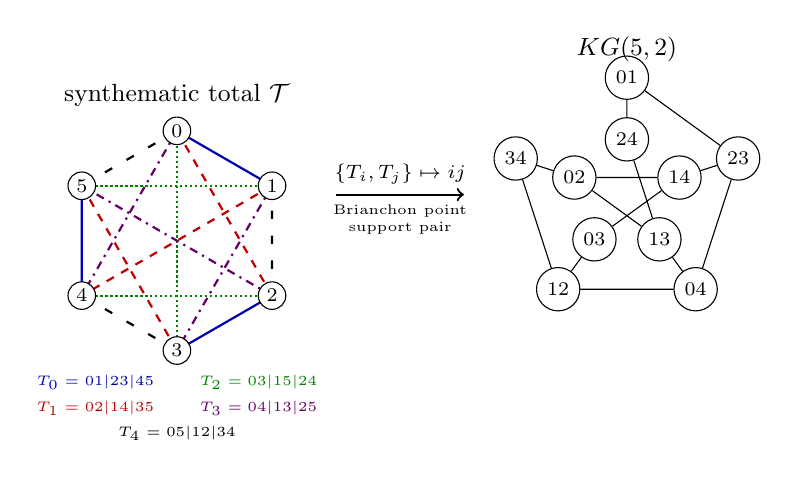
\begin{tikzpicture}[scale=0.9,
  vertex/.style={circle,draw,fill=white,inner sep=1.4pt,font=\scriptsize},
  pvertex/.style={circle,draw,fill=white,minimum size=5.5mm,inner sep=0pt,
                  font=\scriptsize}]
  % The invariant one-factorization on the six coordinate positions.
  \foreach \i/\a in {0/90,1/30,2/-30,3/-90,4/-150,5/150}
    \coordinate (v\i) at (\a:1.55);
  \draw[blue!70!black,thick] (v0)--(v1) (v2)--(v3) (v4)--(v5);
  \draw[red!75!black,thick,dashed] (v0)--(v2) (v1)--(v4) (v3)--(v5);
  \draw[green!50!black,thick,densely dotted] (v0)--(v3) (v1)--(v5) (v2)--(v4);
  \draw[violet!80!black,thick,dash dot] (v0)--(v4) (v1)--(v3) (v2)--(v5);
  \draw[black,thick,loosely dashed] (v0)--(v5) (v1)--(v2) (v3)--(v4);
  \foreach \i in {0,...,5} \node[vertex] at (v\i) {\i};
  \node[font=\small] at (0,2.05) {synthematic total $\mathcal T$};
  \begin{scope}[yshift=-2.0cm,font=\tiny]
    \node[blue!70!black] at (-1.15,0) {$T_0=01|23|45$};
    \node[green!50!black] at (1.15,0) {$T_2=03|15|24$};
    \node[red!75!black] at (-1.15,-.36) {$T_1=02|14|35$};
    \node[violet!80!black] at (1.15,-.36) {$T_3=04|13|25$};
    \node at (0,-.72) {$T_4=05|12|34$};
  \end{scope}

  \draw[->,thick] (2.25,.65)--(4.05,.65)
    node[midway,above,font=\scriptsize] {$\{T_i,T_j\}\mapsto ij$}
    node[midway,below,align=center,font=\tiny] {Brianchon point\\support pair};

  % Petersen graph on the two-subsets of {0,1,2,3,4}; adjacency is disjointness.
  \begin{scope}[xshift=6.35cm,yshift=.65cm]
    \node[pvertex] (p01) at (90:1.65) {01};
    \node[pvertex] (p23) at (18:1.65) {23};
    \node[pvertex] (p04) at (-54:1.65) {04};
    \node[pvertex] (p12) at (-126:1.65) {12};
    \node[pvertex] (p34) at (162:1.65) {34};
    \node[pvertex] (p24) at (90:.78) {24};
    \node[pvertex] (p14) at (18:.78) {14};
    \node[pvertex] (p13) at (-54:.78) {13};
    \node[pvertex] (p03) at (-126:.78) {03};
    \node[pvertex] (p02) at (162:.78) {02};
    \draw (p01)--(p23)--(p04)--(p12)--(p34)--cycle;
    \draw (p01)--(p24) (p23)--(p14) (p04)--(p13)
          (p12)--(p03) (p34)--(p02);
    \draw (p24)--(p13)--(p02)--(p14)--(p03)--cycle;
    \node[font=\small] at (0,2.05) {$KG(5,2)$};
  \end{scope}
\end{tikzpicture}
\caption{The synthematic--Petersen dictionary. The five self-polar
triangles give the displayed perfect matchings. A Petersen vertex $ij$
represents the Brianchon point and complementary support pair attached to
$\{T_i,T_j\}$; two vertices are adjacent when the index pairs are disjoint.}
\label{fig:synthematic-petersen}
\end{figure}

\begin{proposition}[Brianchon--support dictionary]
\label{prop:brianchon-support}
Let $\mathcal T$ be the five self-polar triangles of Edge and
Dye~\cite{Edge1956,Dye1991}, regarded as the five perfect matchings in
their synthematic total, and let $\mathcal B(A)$ be the set of ten
Brianchon points of the Clebsch hexagon. For distinct $T,T'\in\mathcal T$,
the union $T\cup T'$ is an alternating six-cycle. Let $M(T,T')$ be the
perfect matching joining opposite vertices of this cycle, and let
$\beta(T,T')=\{S,S^{\mathsf c}\}$ be its unordered bipartition.
For example, $T_0\cup T_1$ is the cycle
$0,1,4,5,3,2$, and $M(T_0,T_1)=05|13|24$.

The three chords indexed by $M(T,T')$ concur at a point $b(T,T')\in
\mathcal B(A)$. The maps
\[
 \binom{\mathcal T}{2}\longrightarrow\mathcal B(A),
 \qquad \{T,T'\}\longmapsto b(T,T'),
\]
and
\[
 \binom{\mathcal T}{2}\longrightarrow
 \bigl\{\{S,S^{\mathsf c}\}:|S|=3\bigr\},
 \qquad \{T,T'\}\longmapsto\beta(T,T'),
\]
are $A_5$-equivariant bijections. They identify the ten Brianchon points
with the ten complementary support pairs. Under this identification,
Petersen adjacency is disjointness of the corresponding two-element
subsets of $\mathcal T$.
\end{proposition}

\begin{proof}
The opposite-vertex matching is disjoint from $T$ and $T'$ and contains
one edge from each of the other three members of the synthematic total.
Hence $\{T,T'\}$ is recovered as the two members of $\mathcal T$ disjoint
from $M(T,T')$, so the ten triangle pairs give exactly the ten perfect
matchings outside the total. Edge's Clebsch construction says that the
three chords of each such matching concur, at the ten distinct Brianchon
points~\cite[\S\S19--20,30]{Edge1956}. The bipartition bijection and
Petersen assertion are the alternating-cycle construction above.

The ten outside matchings give the ten triple concurrences. The remaining
fifteen intersections of disjoint chords have multiplicity one. Since every
step uses only the invariant total and incidence, both bijections and their
compatibility with the support map are $A_5$-equivariant.
\end{proof}

\begin{corollary}[The decoder reconstructs the Brianchon configuration]
\label{cor:decoder-brianchon}
The ten projective directions having three nearest weight-two errors are
exactly the ten Brianchon points.  At each such direction the three error
supports are pairwise disjoint and hence form a perfect matching of the six
coordinates.  The ten matchings thereby recovered are precisely the ten
perfect matchings outside the five-matching synthematic total.
\end{corollary}

\begin{proof}
The three weight-two representations of a secant-index-three direction use
the three chords through it.  Proposition~\ref{prop:brianchon-support}
identifies the ten triple concurrences with the ten Brianchon points and
their chords with exactly the ten matchings complementary to the total.
\end{proof}

\begin{proposition}[Invariant support chirality]
\label{prop:chirality}
The twenty three-element coordinate supports split into two complementary
$A_5$-orbits $\mathcal O_+$ and $\mathcal O_-$ of size ten. For every
maximum-distance syndrome $s$, each support determines exactly one
weight-three leader of the coset $H^{-1}(s)$; hence that coset has ten
leaders supported in each class. Globally, the $2400$ minimum-weight
leaders split as $1200+1200$.

Every monomial automorphism of $C$ preserves this unordered bipartition.
The other coset in the exotic normalizer $N_{S_6}(A_5)\cong S_5$ exchanges
the two support classes, but its sixty elements are not automorphisms of the
displayed code. Thus the intrinsic structure is an unordered two-class
decomposition, not a canonically signed label. By
Proposition~\ref{prop:brianchon-support}, the ten complementary support
pairs are canonically both the two-subsets of the five self-polar triangles
and the ten Brianchon points.
\end{proposition}

\begin{proof}
The exotic degree-six $A_5$ has two complementary ten-orbits on the $20$
three-supports. It preserves a unique synthematic total, also preserved by
its full $S_5$ normalizer. The alternating-cycle construction of
Figure~\ref{fig:synthematic-petersen} is therefore equivariant, and the
outside normalizer coset exchanges the two support orbits. Fix a
maximum-distance syndrome $s$ and a three-support $S$. The three columns
indexed by $S$ are independent because $A$ is an arc, so they give a unique
coefficient vector representing $s$. None of its three coefficients can
vanish: otherwise $[s]$ would lie on a secant of $A$, contrary to maximum
distance. The resulting error vector therefore has weight three and is the
unique leader with support $S$. Finally, every monomial automorphism induces
a support permutation in $A_5$, by the exact sequence in
Section~\ref{sec:structural}, and so preserves each support orbit. The
outside normalizer coset swaps the two orbits, but the pure-permutation audit
there and the monomial support-image audit show that it does not preserve
$C$, even after coordinate rescaling.
\end{proof}

Equivalently, the two classes form an unbased $\mathbb Z/2$-torsor. This
formulation records the absence of a preferred sign without adding data to
the bipartition.

\begin{remark}[A smaller equivariant decoder]
The stabilizer in
$\operatorname{MAut}(C)$ of one \emph{affine} deep-hole syndrome has order
five and four orbits of size five on its twenty leaders.  Transporting any
one orbit gives a monomial-equivariant set-valued decoder of constant list
size five on the $120$ deep-hole syndromes, and every nonempty equivariant
decoder on this syndrome orbit has list size at least five.  Thus chirality
is not the minimum or coarsest arbitrary equivariant
selection: its two size-ten lists are the proper nonempty selections
determined solely by the support, each a union of two of the size-five
orbits. Exact transport verifies the equivariance statement.
\end{remark}

\section{Why \texorpdfstring{$q=11$}{q=11}}
\label{sec:why11}

The conic-filling syndrome phenomenon of
Sections~\ref{sec:code}--\ref{sec:rigidity} is specific to $q=11$, even
without a symmetry hypothesis on the arc. A universal chord-multiplicity
identity makes this a four-field question, and the only nontrivial residue
is a classical exact-distance problem in the Sylvester graph.

\begin{lemma}[Secant-covering bound]
\label{lem:secant-covering}
Let $A$ be a six-arc of $\PG(2,q)$ disjoint from a nonsingular conic
$\cC$, and suppose $A$ is complete outside $\cC$: every point of
$\PG(2,q)$ lying off $A$ and off $\cC$ lies on some secant of $A$. Then
\[
 15(q-1)\ \ge\ q^2-6,
\]
equivalently $q^2-15q+9\le0$, so $q\le14$.
\end{lemma}

\begin{proof}
Since $A$ has six points and $\cC$ has $q+1$ points, and $A$ is disjoint
from $\cC$,
\[
 \bigl|\PG(2,q)\setminus(A\cup\cC)\bigr|
 = (q^2+q+1)-6-(q+1) = q^2-6.
\]
Each of the $\binom{6}{2}=15$ secants of $A$ is a line of $\PG(2,q)$,
hence has $q+1$ points, exactly two of which lie in $A$; so each secant
covers at most $q-1$ points of $\PG(2,q)\setminus A$, and in particular at
most $q-1$ points of $\PG(2,q)\setminus(A\cup\cC)$. Completeness outside
$\cC$ says the fifteen secants together cover all $q^2-6$ points of this
set, so
\[
 q^2-6\ \le\ 15(q-1).
\]
Overlaps can only reduce the union, so summing the fifteen capacities gives
the required upper bound.
Rearranging, $q^2-15q+9\le0$, whose real roots are
$\tfrac{15\pm\sqrt{189}}2\approx0.62,14.38$; since $q$ is a positive
integer, $q\le14$.
\end{proof}

\begin{lemma}[Chord-defect identity]
\label{lem:chord-defect}
Let $A$ be a six-arc in $\PG(2,q)$, and let $c(A)$ be the number of points
off $A$ incident with three of its fifteen chords. Then
\[
 |\cU(A)|=q^2-14q+55-c(A),\qquad 0\le c(A)\le15.
\]
Consequently, if $|\cU(A)|=q+1$, then
\[
 c(A)=(q-6)(q-9).
\]
\end{lemma}

\begin{proof}
At a point off $A$, concurrent chords have pairwise disjoint endpoint
pairs, so at most three chords occur. Let $n_i$ count the off-arc points on
exactly $i$ chords. Counting chord--point incidences and pairs of chords
with disjoint endpoints gives
\[
 n_1+2n_2+3n_3=15(q-1),\qquad
 n_2+3n_3=\binom{15}{2}-6\binom52=45.
\]
Writing $c(A)=n_3$, the number of covered points off $A$ is
$n_1+n_2+n_3=15q-60+c(A)$. Subtracting this from the
$q^2+q-5$ points off $A$ proves the identity. Each triple concurrence
uses one of the fifteen perfect matchings of the six endpoints, and a fixed
matching can be concurrent at only one point; hence $c(A)\le15$. The last
display follows on setting $|\cU(A)|=q+1$.
\end{proof}

\begin{theorem}[Uniqueness of $q=11$]
\label{thm:why11}
Let $q$ be a prime power. If a six-arc $A\subset\PG(2,q)$ satisfies
$\cU(A)=\cC(\F_q)$ for some nonsingular conic $\cC$, then $q=11$.
Moreover, at $q=11$ every such $A$ is projectively equivalent to the
Clebsch hexagon.
\end{theorem}

\begin{proof}
Lemma~\ref{lem:chord-defect} gives
$c(A)=(q-6)(q-9)$ with $0\le c(A)\le15$. The prime-power condition therefore
leaves only $q\in\{4,5,9,11\}$: the values at $7$ and $8$ are negative,
while every integer $q\ge12$ gives $c(A)\ge18$.

At $q=4$, every six-arc is a hyperoval. Each point off it lies on three
secants (count the six hyperoval points on the five lines through the
point), so $\cU(A)$ is empty. At $q=5$, every six-arc is an oval and hence a
nonsingular conic; the standard internal/external point counts show that
every off-conic point lies on a secant, so again $\cU(A)$ is empty.

It remains to exclude $q=9$. The argument has three steps: the six arc
points must be internal to $\cC$; passant joins of internal points become
distance-two pairs in the Sylvester graph; and that distance graph has
clique number five. Relative to $\cC$,
every chord of $A$ is passant. A point off $\cC$ lies on five passants if it
is internal and four if it is external; hence the five chords through each
vertex force all six vertices of $A$ to be internal. Let $H$ be the graph
on the $36$ internal points, with $P\sim Q$ when $Q\in P^\perp$ under the
conic polarity. Standard conic counts give the intersection array
\[
 \{5,4,2;1,1,4\},
\]
so $H$ is the Sylvester graph
\cite[\S13.1.2]{BrouwerCohenNeumaier1989}; see also the combinatorial
uniqueness proof in~\cite[Thm.~6]{JurisicVidali2019}. For distinct internal
points, the unique possible common neighbor is
$P^\perp\cap Q^\perp=(PQ)^\perp$; consequently $PQ$ is passant exactly when
$P,Q$ are at distance two in $H$. Thus $A$ would be a six-clique in the
exact-distance-two graph of $H$. But its clique number, denoted
$\operatorname{eq}_2(H)$ in
\cite[Table~1]{AbiadJabalAmeliReijnders2025}, is five, a contradiction.

Therefore $q=11$. The final assertion follows from
Theorem~\ref{thm:rigidity}, which puts every matching $q=11$ representative
in the single Clebsch orbit.
\end{proof}

\begin{proposition}[The Clebsch-family uncovered formula]
\label{prop:clebsch-family-uncovered}
Let $H$ be a Clebsch hexagon over $\F_q$. Then
\[
 |\cU(H)|=q^2-14q+45.
\]
If $q\equiv3\pmod4$ and $\cC$ is Dye's associated conic, then
$\cC(\F_q)\subseteq\cU(H)$ and
\[
 |\cU(H)\setminus\cC(\F_q)|=(q-4)(q-11).
\]
In particular, among Clebsch hexagons in this congruence class, the
associated conic is the complete projective deep-hole syndrome locus if and
only if $q=11$.
\end{proposition}

\begin{proof}
Dye defines a Clebsch hexagon by the occurrence of exactly ten Brianchon
points, and his Theorem~1 classifies their existence and projective orbit
\cite[p.~271; Theorem~1, pp.~275--276]{Dye1991}. These points are precisely the off-vertex
triple-chord concurrences counted by $c(H)$
. Thus $c(H)=10$, and
Lemma~\ref{lem:chord-defect} gives
\[
 |\cU(H)|=q^2-14q+55-10=q^2-14q+45.
\]
Dye also shows that the edges of $H$ are non-secants of the associated conic
when $q\equiv3\pmod4$\cite[discussion preceding Theorem~6,
pp.~281--282]{Dye1991}. Hence every rational point of $\cC$ is uncovered.
Subtracting $|\cC(\F_q)|=q+1$ from the first formula gives
\[
 q^2-15q+44=(q-4)(q-11).
\]
The factor vanishes only at $q=4$ and $q=11$, and the stated congruence
leaves only $q=11$. Conversely, Clebsch hexagons exist over $\F_{11}$ by
Dye's Theorem~1, and the inclusion above is then an equality because both
sets have twelve points.
\end{proof}

\begin{remark}[The next admissible field]
At $q=19$, the same icosahedral construction still produces a Clebsch
six-arc disjoint from its associated conic, but the covering fails. The
twenty conic points remain uncovered~\cite[p.~281]{Dye1991}, while
Proposition~\ref{prop:clebsch-family-uncovered} gives
\[
 |\cU(A)|=140=20+120.
\]
Thus $120=(19-4)(19-11)$ additional points escape all fifteen secants, and
$\cU(A)$ lies on no conic. The configuration persists; exact conic filling
is what the factorization isolates at $q=11$.
\end{remark}

\subsection{The small-arc boundary}

The chord moments also put the six-point theorem into a short classification
for all smaller neighboring arc sizes.

\begin{theorem}[Conic-filling loci for $4\le k\le7$]
\label{thm:small-k-conic-filling}
Let $A$ be a $k$-arc in $\PG(2,q)$, where $q$ is a prime power and
$4\le k\le7$. If $\cU(A)$ is the full set of $\F_q$-rational points of a
nonsingular conic, then
\[
 (k,q)=(4,5)\qquad\text{or}\qquad(k,q)=(6,11).
\]
In the first case $A$ is a projective four-frame; in the second it is a
Clebsch hexagon. Conversely, both cases occur.
\end{theorem}

\begin{proof}[Proof with exhaustive finite verification]
Let $n_i$ count off-arc points incident with exactly $i$ chords. For
$k\le7$, at most three pairwise disjoint chords concur. Counting
chord--point incidences and pairs of disjoint chords gives the two universal
moments
\[
 \sum_i i n_i=\binom{k}{2}(q-1),\qquad
 \sum_i\binom{i}{2}n_i=3\binom{k}{4}.
\]
For $k=4$, the second moment forces $n_2=3$, and hence
$|\cU(A)|=(q-2)(q-3)$. Equating this with $q+1$ gives $q=5$. Every
four-arc is a projective frame, and for the standard frame a direct
substitution gives
\[
 \cU(A)=Z(X^2+Y^2+Z^2+XY+XZ+YZ),
\]
a nonsingular six-point conic. For $k=5$, the same moments force
$n_2=15$ and $|\cU(A)|=q^2-9q+21$; equality with $q+1$ would require
$q^2-10q+20=0$, which has no integral root. The case $k=6$ is
Theorem~\ref{thm:why11} together with Theorem~\ref{thm:rigidity}.

For $k=7$, the moments give
\[
 |\cU(A)|=q^2-20q+120-n_3.
\]
If this equals $q+1$, then
\[
 n_3=q^2-21q+119,\quad
 n_2=105-3n_3,\quad
 n_1=3(q^2-14q+42).
\]
The standard arc-size bound gives $q\ge7$.  The condition $n_2\ge0$ gives
$q\le15$, so the prime-power candidates are
$q\in\{7,8,9,11,13\}$; then $n_1\ge0$ eliminates $7,8,9$.
Thus only $q=11$ and $q=13$ remain, with forced spectra
$(n_1,n_2,n_3)=(27,78,9)$ and $(87,60,15)$ respectively. An exhaustive
four-frame-normalized enumeration now supplies the finite exclusion. It
finds no conic-filling seven-arc in
either plane. Every seven-arc is reached because it contains a four-frame;
equivalently, extending every normalized six-arc by each point of its
uncovered locus produces every resulting seven-arc exactly three times,
according to which non-frame point is deleted. For
all candidates with $|\cU(A)|=q+1$, the quadratic evaluation matrix has
full rank six.
\end{proof}

For $k\ge8$ the second moment leaves additional concurrency parameters, so
the analogous classification remains open.

\section{Verification architecture}
\label{sec:verification}

Table~\ref{tab:verification} separates cited input, kernel-checked finite
certificates, and fail-closed enumeration. Lean and script paths are
relative to \path{lean/RelativeConicArcs/} and the paper directory;
commands, hashes, sentinels, and import closures will accompany the archive.

\begin{table}[H]
\centering
\tiny
\begin{tabular}{@{}>{\raggedright\arraybackslash}p{0.17\textwidth}
                    >{\raggedright\arraybackslash}p{0.21\textwidth}
                    >{\raggedright\arraybackslash}p{0.25\textwidth}
                    >{\raggedright\arraybackslash}p{0.27\textwidth}@{}}
\toprule
Result & Cited or proved input & Lean certificate & Executable replay \\
\midrule
$A_5$ orbits and syndrome conic
& Dye; Proposition~\ref{prop:a5-point-orbits}
& \path{Q11A5PointOrbits.lean}; \path{Q11Coding.lean}
& \path{check_rigidity_degenerate_conic.py} \\
Decoding and chirality
& arc--coset dictionary; Edge--Dye triangles
& \path{Q11DecodingSynthesis.lean}
& \path{check_decoding.py}; \path{check_chirality.py};
\path{check_code_automorphisms.py} \\
Rigidity theorem
& line bound; chord defect; Dye's Theorem~1
& \path{Q11DyeAxioms.lean}; \path{Q11DyeConsequences.lean};
\path{SixArcDefectBridge.lean}
& $1548$-representative rigidity replay \\
Gap and low-degree loci
& finite linear algebra over $\F_{11}$
& ---
& \path{check_global_conic_gap.py}; \path{check_perturbation_gap.py};
\path{check_low_degree_loci.py}; Singular replay \\
Uniqueness of $q=11$
& chord moments; cited Sylvester bound
& \path{ClebschChordDefect.lean}; \path{Q9Sylvester.lean}
& \path{check_small_q_uniqueness.py}; from-scratch $q=9$ certificate \\
Clebsch-family formula
& Dye's ten Brianchon points and edge criterion
& ---
& \path{check_q19_nonexample.py} \\
The range $4\le k\le7$
& two universal chord moments
& \path{SmallKChordMoments.lean}; \path{SmallKGeometricBridge.lean}
& \path{check_small_k_conic_filling.py} \\
\bottomrule
\end{tabular}
\caption{Trust and verification map for the principal results.}
\label{tab:verification}
\end{table}

The formal development axiomatizes exactly two consequences of Dye's
Theorem~1: the ten-point Brianchon bound and the classification of equality.
The line bound and chord-defect identity are proved independently. At
$q=11$, the finite census also checks the imported numerical conclusion:
$|\cU(A)|=12=22-10$ is equivalent to the maximal value $c(A)=10$.

\subsection{Independent small-field census}

Normalizing an ordered four-frame and enumerating the remaining unordered
pair gives the following exact check. Exponents record multiplicities.

\begin{center}
\small
\begin{tabular}{@{}r r l r@{}}
\toprule
$q$ & representatives & histogram of $|\cU(A)|$ & conic matches\\
\midrule
2  & 0    & --- & 0\\
3  & 0    & --- & 0\\
4  & 1    & $0^1$ & 0\\
5  & 3    & $0^3$ & 0\\
7  & 70   & $0^{40},2^{30}$ & 0\\
8  & 195  & $0^{45},4^{150}$ & 0\\
9  & 441  & $0^6,4^{15},6^{120},7^{120},8^{180}$ & 0\\
11 & 1548 & $12^6,16^{30},18^{150},19^{300},20^{630},21^{360},22^{72}$ & 6\\
13 & 4015 & $36^{85},38^{210},39^{480},40^{1080},41^{1800},42^{360}$ & 0\\
\bottomrule
\end{tabular}
\end{center}

The replay uses exact arithmetic in every field and tests both nonsingular
and singular conic forms in characteristic two. A separate $q=9$
certificate constructs the polarity graph, verifies the passant/distance-two
dictionary, and computes clique number five.

\section{Conclusion}

The Clebsch code shows that covering-radius data can recover geometry that
was not built into the code: conic containment of the deep-hole directions
forces the Clebsch hexagon and hence its $A_5$ symmetry. The proof separates
the mechanism from the census. A line bound and a chord-defect identity
reduce the geometric condition to Dye's equality case; enumeration is
needed only for the sharp numerical gap and its refinements.

The same chord moments explain both the isolation of $q=11$ and the
classification for $4\le k\le7$. For $k\ge8$, further concurrency moments
are needed. Other concrete problems are to exhaust the degree-six kernels
from Remark~\ref{rem:degree-threshold} and to connect fixed-$k$ rigidity
with the large-arc conic-forcing regime. These are tests of how far a
syndrome locus can reconstruct the projective system that produced it.

\bibliographystyle{plain}
\begin{thebibliography}{99}

\bibitem{BSW1992}
A.~Blokhuis, Á.~Seress, and H.~A.~Wilbrink,
\newblock Characterization of complete exterior sets of conics,
\newblock \emph{Combinatorica} \textbf{12}(2) (1992), 143--147.
\newblock doi:10.1007/BF01204717.

\bibitem{BicharaKorchmaros1982}
A.~Bichara and G.~Korchm\'aros,
\newblock Note on $(q+2)$-sets in a Galois plane of order $q$,
\newblock in \emph{Combinatorial and Geometric Structures and Their
Applications}, Annals of Discrete Mathematics \textbf{14}, North-Holland,
1982, 117--121.
\newblock doi:10.1016/S0304-0208(08)73588-6.

\bibitem{Clebsch1871}
A.~Clebsch,
\newblock Ueber die Anwendung der quadratischen Substitution auf die
Gleichungen 5-ten Grades und die geometrische Theorie des ebenen Fünfseits,
\newblock \emph{Mathematische Annalen} \textbf{4} (1871), 284--345.

\bibitem{Edge1956}
W.~L.~Edge,
\newblock Conics and orthogonal projectivities in a finite plane,
\newblock \emph{Canadian Journal of Mathematics} \textbf{8} (1956), 362--382.

\bibitem{DrakeKeating2004}
D.~A.~Drake and K.~Keating,
\newblock Ovals and hyperovals in Desarguesian nets,
\newblock \emph{Designs, Codes and Cryptography} \textbf{31} (2004),
195--212.
\newblock \url{https://doi.org/10.1023/B:DESI.0000015883.89954.80};
arXiv:math/0202115.

\bibitem{ArcsCompleteOutsideConic}
T.~Rudd,
\newblock Arcs complete outside a prescribed conic: a prescribed-hole
defect identity and a certified classification over $\F_{16}$,
\newblock working paper, 2026.

\bibitem{ChengMurray2007}
Q.~Cheng and E.~Murray,
\newblock On deciding deep holes of Reed--Solomon codes,
\newblock in \emph{Theory and Applications of Models of Computation (TAMC
2007)}, Lecture Notes in Computer Science \textbf{4484}, Springer, 2007,
296--305.

\bibitem{DMP2021}
A.~A.~Davydov, S.~Marcugini, and F.~Pambianco,
\newblock On the weight distribution of the cosets of MDS codes,
\newblock \emph{Advances in Mathematics of Communications} \textbf{17}(5)
(2023), 1115--1138.
\newblock arXiv:2101.12722v2.
\newblock (Numbered results are cited by their arXiv~v2 numbering.)

\bibitem{AbiadJabalAmeliReijnders2025}
A.~Abiad, A.~Jabal Ameli, and L.~Reijnders,
\newblock The clique number of the exact distance $t$-power graph:
complexity and eigenvalue bounds,
\newblock \emph{Discrete Applied Mathematics} \textbf{363} (2025), 55--70.
\newblock doi:10.1016/j.dam.2024.11.032.

\bibitem{BrouwerCohenNeumaier1989}
A.~E.~Brouwer, A.~M.~Cohen, and A.~Neumaier,
\newblock \emph{Distance-Regular Graphs},
\newblock Ergebnisse der Mathematik und ihrer Grenzgebiete, vol.~18,
Springer-Verlag, Berlin, 1989.

\bibitem{JurisicVidali2019}
A.~Juri\v{s}i\'c and J.~Vidali,
\newblock The Sylvester graph and Moore graphs,
\newblock \emph{European Journal of Combinatorics} \textbf{80} (2019),
184--193.
\newblock doi:10.1016/j.ejc.2018.02.018.

\bibitem{Dye1991}
R.~H.~Dye,
\newblock Hexagons, conics, $A_5$ and $\mathrm{PSL}_2(K)$,
\newblock \emph{Journal of the London Mathematical Society} (2) \textbf{44}
(1991), 270--286.
\newblock doi:10.1112/jlms/s2-44.2.270.

\bibitem{DromsMellingerMeyer2006}
S.~V.~Droms, K.~E.~Mellinger, and C.~Meyer,
\newblock LDPC codes generated by conics in the classical projective plane,
\newblock \emph{Designs, Codes and Cryptography} \textbf{40} (2006),
343--356.
\newblock doi:10.1007/s10623-006-0022-6.

\bibitem{GuruswamiVardy2005}
V.~Guruswami and A.~Vardy,
\newblock Maximum-likelihood decoding of Reed--Solomon codes is NP-hard,
\newblock \emph{IEEE Transactions on Information Theory} \textbf{51}(7)
(2005), 2249--2256.

\bibitem{Hirschfeld1998}
J.~W.~P.~Hirschfeld,
\newblock \emph{Projective Geometries over Finite Fields}, second edition,
\newblock Oxford University Press, 1998.

\bibitem{MadisonWu2012}
A.~L.~Madison and J.~Wu,
\newblock On binary codes from conics in $\PG(2,q)$,
\newblock \emph{European Journal of Combinatorics} \textbf{33} (2012),
33--48.
\newblock doi:10.1016/j.ejc.2011.08.001; arXiv:1104.0324.

\bibitem{MadisonWu2016}
A.~L.~Madison and J.~Wu,
\newblock Conics arising from external points and their binary codes,
\newblock \emph{Designs, Codes and Cryptography} \textbf{78} (2016),
473--491.
\newblock doi:10.1007/s10623-014-0013-y.

\bibitem{NgWild2001}
S.-L.~Ng and P.~R.~Wild,
\newblock On $k$-arcs covering a line in finite projective planes,
\newblock \emph{Ars Combinatoria} \textbf{58} (2001), 289--300.

\bibitem{SadehThesis1984}
A.~R.~Sadeh,
\newblock \emph{Classification of $k$-arcs in $\PG(2,11)$ and cubic
surfaces in $\PG(3,11)$},
\newblock D.Phil.\ thesis, University of Sussex, 1984.

\bibitem{SinWuXiang2011}
P.~Sin, J.~Wu, and Q.~Xiang,
\newblock Dimensions of some binary codes arising from a conic in
$\PG(2,q)$,
\newblock \emph{Journal of Combinatorial Theory, Series A} \textbf{118}
(2011), 853--878.
\newblock doi:10.1016/j.jcta.2010.11.010; arXiv:0911.2018.

\bibitem{StormeThas1991}
L.~Storme and J.~A.~Thas,
\newblock Generalized Reed--Solomon codes and normal rational curves: an
improvement of results by Seroussi and Roth,
\newblock in \emph{Advances in Finite Geometries and Designs}, Oxford
University Press, 1991, 369--389.

\bibitem{SVM1995}
L.~Storme and H.~Van~Maldeghem,
\newblock Primitive arcs in $\PG(2,q)$,
\newblock \emph{Journal of Combinatorial Theory, Series A} \textbf{69}
(1995), 200--216.
\newblock doi:10.1016/0097-3165(95)90051-9.

\bibitem{Wu2013}
J.~Wu,
\newblock Conics arising from internal points and their binary codes,
\newblock \emph{Linear Algebra and its Applications} \textbf{439} (2013),
422--434.
\newblock doi:10.1016/j.laa.2013.04.004.

\bibitem{ZWK2020}
Y.~Zhang, D.~Wan, and K.~Kaipa,
\newblock Deep holes of projective Reed--Solomon codes,
\newblock \emph{IEEE Transactions on Information Theory} \textbf{66}(4)
(2020), 2392--2401.
\newblock arXiv:1901.05445.

\end{thebibliography}

\end{document}
